% \iffalse
\let\negmedspace\undefined
\let\negthickspace\undefined
\documentclass[journal,12pt,twocolumn]{IEEEtran}
\usepackage{cite}
\usepackage{amsmath,enumitem,amssymb,amsfonts,amsthm}
\usepackage{algorithmic}
\usepackage{graphicx}
\usepackage{float}
\usepackage{textcomp}
\usepackage{xcolor}
\usepackage{caption}
\usepackage{txfonts}
\usepackage{listings}
\usepackage{enumitem}
\usepackage{mathtools}
\usepackage{gensymb}
\usepackage{comment}
\usepackage[breaklinks=true]{hyperref}
\usepackage{tkz-euclide} 
\usepackage{listings}
\usepackage{gvv}                                        
\def\inputGnumericTable{}                                 
\usepackage[latin1]{inputenc}                              
\usepackage{color}                                            
\usepackage{array}                                            
\usepackage{longtable}                                       
\usepackage{calc}                                             
\usepackage{multirow}                                         
\usepackage{hhline}                                           
\usepackage{ifthen}                                        
\usepackage{lscape}
\newtheorem{theorem}{Theorem}[section]
\newtheorem{problem}{Problem}
\newtheorem{proposition}{Proposition}[section]
\newtheorem{lemma}{Lemma}[section]
\newtheorem{corollary}[theorem]{Corollary}
\newtheorem{example}{Example}[section]
\newtheorem{definition}[problem]{Definition}
\newcommand{\BEQA}{\begin{eqnarray}}
\newcommand{\EEQA}{\end{eqnarray}}
\newcommand{\define}{\stackrel{\triangle}{=}}
\theoremstyle{remark}
\newtheorem{rem}{Remark}
\begin{document}



\bibliographystyle{IEEEtran}
\vspace{3cm}

\title{NCERT 11.9.5 26Q}
\author{EE23BTECH11015 - DHANUSH V NAYAK$^{*}$% <-this % stops a space
}
\maketitle
\newpage
\bigskip

\renewcommand{\thefigure}{\theenumi}
\renewcommand{\thetable}{\theenumi}

\bibliographystyle{IEEEtran}
\textbf{Question:} Show that
\begin{align}
    \frac{1\times2^2 + 2\times3^2 + \dots + n\times(n+1)^2}{1^2\times2 + 2^2\times3 + \dots + n^2\times(n+1)}  = \frac{3n+5}{3n+1}\notag
\end{align}
\textbf{Solution:}
\begin{enumerate}[label=\arabic*.]
\item Consider the Numerator of the LHS part:
\begin{align}
    1\times2^2 + 2\times3^2 + \dots + n\times(n+1)^2 = \sum_{k=1}^n k(k+1)^2 
\end{align}

Now,
\begin{align}
    \sum_{k=1}^n k\brak{k+1}^2 &= \sum_{k=1}^n k^3+2k^2+k\\
                          &=  \sum_{k=1}^n k^3 + \sum_{k=1}^n 2k^2 + \sum_{k=1}^n k\\
                          &=  \sum_{k=1}^n k^3 + 2\sum_{k=1}^n k^2 + \sum_{k=1}^n k\\
                          &= \left(\frac{n\brak{n+1}}{2}\right)^{\scriptstyle 2} + 2\cdot \frac{n\brak{n+1}\brak{2n+1}}{6}\\  &+\frac{n\brak{n+1}}{2}\notag \\
                          &= \frac{n\brak{n+1}}{2}\left[\frac{n\brak{n+1}}{2} + \frac{2}{3}\brak{2n+1} + 1\right]\\
                          &= \frac{n\brak{n+1}}{2}\left[\frac{3n^2 + 11n +10}{6}\right]\\
                          &= \frac{n\brak{n+1}}{12}\left[3n^2 + 6n + 5n + 10\right]\\
                          &= \frac{n\brak{n+1}}{12}\left[3n\brak{n+2}+5\brak{n+2}\right]\\
                          &= \frac{n\brak{n+1}\brak{n+2}\brak{3n+5}}{12}
\end{align}
Therefore,
\begin{equation}
   1\times2^2 + 2\times3^2 + \dots + n\times\brak{n+1}^2 = \frac{n\brak{n+1}\brak{n+2}\brak{3n+5}}{12}   \\
\end{equation}

\begin{table}[H]
\centering
  \renewcommand\thetable{1}
\setlength{\extrarowheight}{9pt}
\resizebox{0.54\textwidth}{!}{
\begin{tabular}{|c|c|c|}
\hline
\textbf{Parameter} & \textbf{Description} & \textbf{Value} \\ \hline
$n$ & Integer & 1, 2, 3, 4, ... \\ \hline
$x_1(n)$ & Numerator sequence & $\brak{n^{3} + 5n^{2} + 20n + 4} \cdot u\brak{n}$ \\ \hline
$x_2(n)$ & Denominator sequence & $\brak{n^{3}+4n^{2}+5n+2}\cdot u\brak{n}$ \\ \hline
$X_1(z)$ & z-transform of $x_1(n)$ & $\frac{4+14z^{-1}-24z^{-2}+12z^{-3}}{\brak{1-z^{-1}}^4} , \cbrak{z\in\mathbb{C} : \lvert z \rvert > 1} $ \\ \hline
$X_2(z)$ & z-transform of $x_2(n)$ & $\frac{2+4z^{-1}}{\brak{1-z^{-1}}^4},\cbrak{z\in\mathbb{C} : \lvert z \rvert > 1}  $ \\ \hline
$U(z)$ & z-transform of $u(n)$ & $\frac{1}{1 - z^{-1}},\cbrak{z\in\mathbb{C} : \lvert z \rvert > 1}  $ \\ \hline
ROC & Region of convergence & $\left\{ z : \left|\sum_{n=-\infty}^{\infty} x(n)z^{-n}\right| < \infty \right\}$ \\ \hline
$X_k(z)$ & z-transform of $n^k u(n)$ & $\brak{-z}^k \frac{d^kU\brak{z}}{dz^k} , \hspace{4pt}\cbrak{z\in\mathbb{C} : \lvert z \rvert > 1} $ \\ \hline
$X_1\brak{z}$ & z-transform of $n\cdot u\brak{n}$ & $\frac{z^{-1}}{\brak{1-z^{-1}}^2}  , \hspace{4pt} \cbrak{z\in\mathbb{C} : \lvert z \rvert > 1} $ \\ \hline 
$X_2\brak{z}$ & z-transform of $n^{2}\cdot u\brak{n}$ & $\frac{z^{-1}\brak{z^{-1}+1}}{\brak{1-z^{-1}}^3} , \hspace{4pt} \cbrak{z\in\mathbb{C} : \lvert z \rvert > 1} $ \\ \hline 
$X_3\brak{z}$ & z-transform of $n^{3}\cdot u\brak{n}$ & $\frac{z^{-1}\brak{1+4z^{-1}+z^{-2}}}{\brak{1-z^{-1}}^4}, \hspace{4pt} \cbrak{z\in\mathbb{C} : \lvert z \rvert > 1} $ \\ \hline 
$X_4\brak{z}$ & z-transform of $n^{4}\cdot u\brak{n}$ & $\frac{z^{-1}\brak{1+11z^{-1}+11z^{-2}+z^{-3}}}{\brak{1-z^{-1}}^5}, \hspace{4pt} \cbrak{z\in\mathbb{C} : \lvert z \rvert > 1} $ \\ \hline 
\end{tabular}}
\caption{Parameter Table}
\label{tab:11.9.5.26.1}
\end{table}


\begin{align}
\frac{\brak{n+1}\brak{n+2}\brak{n+3}\brak{3n+8}}{12}\cdot u\brak{n} &= x\brak{n}
\end{align}
    
\begin{align}
     x\brak{n} & = \begin{cases}
        0 & \text{for } n < 0 \\
         \frac{\brak{n+1}\brak{n+2}\brak{n+3}\brak{3n+8}}{12}& \text{for } n \geq 0
    \end{cases}
\end{align}
\begin{figure}[h]
    \hspace{1cm}
    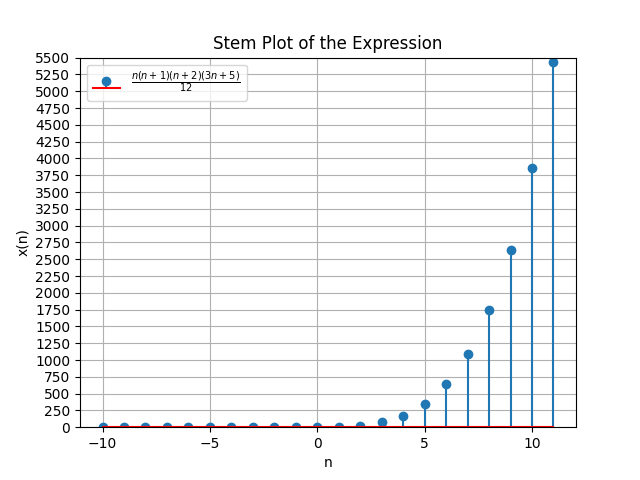
\includegraphics[width=1\columnwidth]{Figure_1.png}
    \caption{Stem Plot of $x\brak{n}$}
\end{figure}
    
Derivation of z-transform of numerator :
\begin{align}
    x\brak{n} &=  \frac{\brak{n+1}\brak{n+2}\brak{n+3}\brak{3n+8}}{12}\cdot u\brak{n}\\
         &= \frac{3n^4 + 26n^3 + 81n^2 + 106n + 48}{12}\cdot u\brak{n} \label{eq:11.9.5.26.1}
\end{align}
    \begin{align}
    X\brak{z} &= \sum_{n=-\infty}^\infty x\brak{n}z^{-n}\\
U\brak{z} &= \sum_{n=-\infty}^{\infty} u\brak{n}\cdot z^{-n} 
    \end{align}
\begin{align}
    u(n) = \begin{cases}
        0 & \text{for } n < 0 \\
        1 & \text{for } n \geq 0\\
    \end{cases}
\end{align}
\begin{align}
    U\brak{z} &= \sum_{n=0}^{\infty} \brak{1} \cdot z^{-n} \\
     &= 1 + z^{-1} + z^{-2} + \ldots \\
     &= \frac{1}{1 - z^{-1}} 
\end{align}

By the differentiation property:\\
\begin{align}
x\brak{n} &\stackrel{\mathcal{Z}}{\longleftrightarrow} X\brak{z}\\
n^k x\brak{n} &\stackrel{\mathcal{Z}}{\longleftrightarrow} \brak{-z}^k \frac{d^kX\brak{z}}{dz^k}\\
n^k u\brak{n} &\stackrel{\mathcal{Z}}{\longleftrightarrow} \brak{-z}^k \frac{d^kU\brak{z}}{dz^k}
\end{align}
\begin{align} \label{eq:a}
    X_k\brak{z} =  \brak{-z}^k \frac{d^kU\brak{z}}{dz^k}
\end{align}
For the Z-transform of $n \cdot u\brak{n}$, 
\text{ substituting } k=1 \text{ in Equation \eqref{eq:a}:}
\begin{align}
    X_1\brak{z} &=  \brak{-z} \frac{dU\brak{z}}{dz}\\
    \frac{dU\brak{z}}{dz} &= -\frac{z^{-2}}{\brak{1-z^{-1}}^2}, \\
    X_1\brak{z} &= \frac{z^{-1}}{\brak{1-z^{-1}}^2}.
\end{align}
\text{Similarly , substituting } k=2,3,4 in equation \eqref{eq:a}:
\begin{align}
     X_2\brak{z} &= \frac{z^{-1}\brak{z^{-1}+1}}{\brak{1-z^{-1}}^3}\\
     X_3\brak{z} &= \frac{z^{-1}\brak{1+4z^{-1}+z^{-2}}}{\brak{1-z^{-1}}^4}\\
    X_4\brak{z} &= \frac{z^{-1}\brak{1+11z^{-1}+11z^{-2}+z^{-3}}}{\brak{1-z^{-1}}^5} 
\end{align}
The Region of Convergence \brak{ROC} is defined as the set of points in the complex plane for which the Z-transform summation converges, i.e., doesn't blow up in magnitude to infinity:
The Region of Convergence \brak{ROC} is defined as:
\begin{equation}\label{eq:roc_definition}
    \text{ROC} = \left\{ z : \left\lvert \sum_{n=-\infty}^{\infty} x\brak{n}z^{-n} \right\rvert < \infty \right\}
\end{equation}


Equation \eqref{eq:roc_definition} expresses the set of points in the complex plane for which the Z-transform summation converges.

The Z-transform of the unit step signal $u\brak{n}$ is given by:
\begin{equation}\label{eq:z_transform}
    U\brak{z} = \sum_{n=-\infty}^{\infty} u\brak{n} z^{-n}
\end{equation}
\begin{align}
    u(n) = \begin{cases}
        0 & \text{for } n < 0 \\
        1 & \text{for } n \geq 0\\
    \end{cases}
\end{align}
\begin{align}
    U\brak{z} = \sum_{n=0}^{\infty} z^{-n}\label{eq:z_transform_simplified}
\end{align}
\begin{equation}
    \text{ROC} = \left\{ z : \left\lvert \sum_{n=0}^{\infty}z^{-n} \right\rvert < \infty \right\}
\end{equation}
This is an infinite GP. And it converges only if $|r|<1$ where r is the common ratio.And here , $|r|=|z^{-1}|$ Therefore,
the Region of Convergence \brak{ROC} for this Z-transform is:
\begin{equation}
    \text{ROC: } |z| > 1
\end{equation}
In the differentiation property, ROC does not change:\\
\begin{align}
x\brak{n} &\stackrel{\mathcal{Z}}{\longleftrightarrow} X\brak{z},\hspace{4pt} ROC = R\\
n^k x\brak{n} &\stackrel{\mathcal{Z}}{\longleftrightarrow} \brak{-z}^k \frac{d^kX\brak{z}}{dz^k},\hspace{4pt} ROC = R 
\end{align}
Therefore,
\begin{align}
    X_1\brak{z} &= \frac{z^{-1}}{\brak{1-z^{-1}}^2} , \hspace{4pt} ROC=|z|>1\\
    X_2\brak{z} &= \frac{z^{-1}\brak{z^{-1}+1}}{\brak{1-z^{-1}}^3} , \hspace{4pt} ROC=|z|>1\\
    X_3\brak{z} &= \frac{z^{-1}\brak{1+4z^{-1}+z^{-2}}}{\brak{1-z^{-1}}^4}, \hspace{4pt} ROC=|z|>1\\
    X_4\brak{z} &= \frac{z^{-1}\brak{1+11z^{-1}+11z^{-2}+z^{-3}}}{\brak{1-z^{-1}}^5}, \hspace{4pt} ROC=|z|>1
\end{align}
\text{Z-Transform of Equation \eqref{eq:11.9.5.26.1} can be written as:} 
\begin{align}
X\brak{z} &= \frac{1}{12}\brak{3X_4\brak{z} + 26X_3\brak{z} + 81X_2\brak{z} + 106X_1\brak{z}} \label{eq:11.9.5.26.2} \notag \\
&\quad + 48U \brak{z} \\
&= \frac{3}{12}\left(\frac{z^{-1}\brak{1+11z^{-1}+11z^{-2}+z^{-3}}}{\brak{1-z^{-1}}^5}\right) \notag \\
&\quad + \frac{26}{12}\left(\frac{z^{-1}\brak{1+4z^{-1}+z^{-2}}}{\brak{1-z^{-1}}^4}\right) \\
&\quad + \frac{81}{12}\left(\frac{z^{-1}\brak{z^{-1}+1}}{\brak{1-z^{-1}}^3}\right) \notag \\
&\quad + \frac{106}{12}\left(\frac{z^{-1}}{\brak{1-z^{-1}}^2}\right) + \frac{48}{12}\left(\frac{1}{1 - z^{-1}} \right) \notag \\
&= \frac{24 \brak{z^4} \brak{2z+1}}{\brak{z-1}^5}
\end{align}


Consider the linear combination of two signals in the time domain:
\begin{align}
    a_1 x_1\brak{n} + a_2 x_2\brak{n} &\stackrel{\mathcal{Z}}{\longleftrightarrow} a_1 X_1\brak{z} + a_2 X_2\brak{z} \label{eq:combined_signal}\\
    \text{ROC} &= \text{ROC}_1 \cap \text{ROC}_2 \label{eq:roc_intersection}
\end{align}
Therefore, ROC of equation\eqref{eq:11.9.5.26.2} is the intersection of the ROC of each signal. Every signal has ROC $|z|>1$. So,
\begin{align}
    \text{ROC of $X\brak{z}$} \text{\hspace{3pt}is\hspace{3pt}} |z|>1
\end{align}

\item Consider the Denominator of the RHS part:
\begin{equation}
    1^2\times2 + 2^2\times3 +\dots + n^2\times\brak{n+1} = \sum_{k=1}^n k^2\brak{k+1}
\end{equation}
Now,
\begin{align}
     \sum_{k=1}^n k^2\brak{k+1} &= \sum_{k=1}^n k^3+k^2\\
                           &=  \sum_{k=1}^n k^3 + \sum_{k=1}^n k^2\\
                           &=  \left(\frac{n\brak{n+1}}{2}\right)^{\scriptstyle 2}+\frac{n\brak{n+1}\brak{2n+1}}{6}\\ 
                           &= \frac{n\brak{n+1}}{2}\left[\frac{n\brak{n+1}}{2} +\frac{2n+1}{3}\right]\\
                           &= \frac{n\brak{n+1}}{2}\left[\frac{3n^2+7n+2}{6}\right]\\
                           &= \frac{n\brak{n+1}}{12}\left[3n^2+6n + n+2\right]\\
                           &= \frac{n\brak{n+1}}{12}\left[3n\brak{n+2}+\brak{n+2}\right]\\
                           &= \frac{n\brak{n+1}\brak{n+2}\brak{3n+1}}{12}
\end{align}
\begin{align}
    \frac{\brak{n+1}\brak{n+2}\brak{n+3}\brak{3n+4}}{12}\cdot u\brak{n} &= y\brak{n}
\end{align}
\begin{align}
     y\brak{n} & = \begin{cases}
        0 & \text{for } n < 0 \\
        \frac{\brak{n+1}\brak{n+2}\brak{n+3}\brak{3n+4}}{12}\cdot& \text{for } n \geq 0
    \end{cases}
\end{align}
\begin{figure}[h]
    \centering
    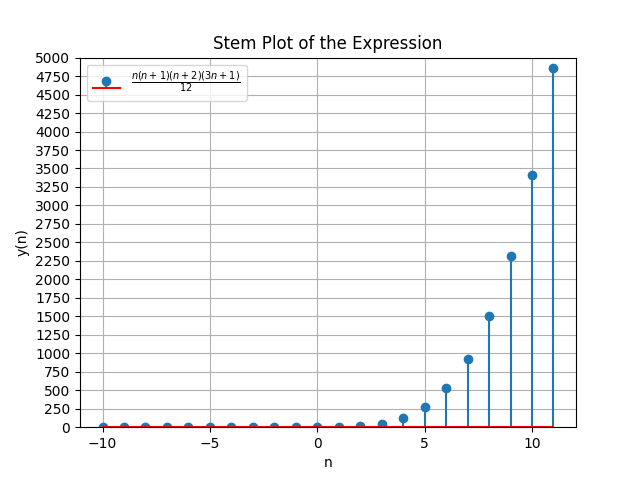
\includegraphics[width=\columnwidth]{Figure_2.png}
    \caption{Stem Plot of $y\brak{n}$}
\end{figure}
\vspace{1cm}

\begin{align}
     \dfrac{ \sum_{k=1}^n k\brak{k+1}^2 }{\sum_{k=1}^n k^2\brak{k+1}} &= \dfrac{\frac{n\brak{n+1}\brak{n+2}\brak{3n+5}}{12}}{\frac{n\brak{n+1}\brak{n+2}\brak{3n+1}}{12}}\\
                                                            &= \frac{3n+5}{3n+1}
\end{align}

Derivation of z-transform of the denominator:
\begin{align}
    y\brak{n} &= \frac{\brak{n+1}\brak{n+2}\brak{n+3}\brak{3n+4}}{12}\cdot u\brak{n}\\
         &= \frac{3n^4 + 22n^3 + 57n^2 + 62n + 24}{12}\cdot u\brak{n} \label{eq:11.9.5.26.3}
\end{align}

\begin{equation}
    Y\brak{z} = \sum_{n=-\infty}^\infty y\brak{n}\cdot z^{-n}
\end{equation}
We can say that $Y_k\brak{z}$ denote the z-transform of $n^{k}u\brak{n}$ which will be same as respective $X_k\brak{z}$.
\begin{align}\label{eq:61}
    X_k&=Y_k\\
    Y_k\brak{z} &=  \brak{-z}^k \frac{d^kU\brak{z}}{dz^k}\label{eq:24}
\end{align}
Now substituting k=1,2,3,4 we get :
\begin{align}
    Y_1\brak{z} &= \frac{z^{-1}}{\brak{1-z^{-1}}^2} , \hspace{4pt} ROC=|z|>1\\
    Y_2\brak{z} &= \frac{z^{-1}\brak{z^{-1}+1}}{\brak{1-z^{-1}}^3} , \hspace{4pt} ROC=|z|>1\\
    Y_3\brak{z} &= \frac{z^{-1}\brak{1+4z^{-1}+z^{-2}}}{\brak{1-z^{-1}}^4}, \hspace{4pt} ROC=|z|>1\\
    Y_4\brak{z} &= \frac{z^{-1}\brak{1+11z^{-1}+11z^{-2}+z^{-3}}}{\brak{1-z^{-1}}^5}, \hspace{4pt} ROC=|z|>1
\end{align}
\text{Z-Transform of equation\eqref{eq:11.9.5.26.3} }
\begin{align}
    Y\brak{z} &=\frac{1}{12}\brak{3Y_4\brak{z} + 22Y_3\brak{z} + 57Y_2\brak{z} + 62Y_1\brak{z}} \\ 
&\quad + 24U\brak{z} \notag  \\
         &= \frac{3}{12}\left(\frac{z^{-1}\brak{1+11z^{-1}+11z^{-2}+z^{-3}}}{\brak{1-z^{-1}}^5}\right)\\ &+ \frac{22}{12}\left(\frac{z^{-1}\brak{1+4z^{-1}+z^{-2}}}{\brak{1-z^{-1}}^4}\right) 
         + \frac{57}{12}\left(\frac{z^{-1}\brak{z^{-1}+1}}{\brak{1-z^{-1}}^3}\right)\notag \\ &+ \frac{62}{12}\left(\frac{z^{-1}}{\brak{1-z^{-1}}^2}.\right)+ \frac{24}{12}\left(\frac{1}{1 - z^{-1}} \right) \notag \\
         &= \frac{24 \brak{z^4} \brak{2z+1}}{\brak{z-1}^5}
\end{align}
$Y\brak{z}$ is a linear combination of $Y_k\brak{z}$ for $k=1,2,3,4$
\begin{align}
    Y\brak{z} &= a_1 Y_1\brak{z} + a_2 Y_2\brak{z} + a_3 Y_3\brak{z} + a_4 Y_4\brak{z} \label{eq:linear_combination_Y} \\
    \text{ROC}_{Y} &= \text{ROC}_{1} \cap \text{ROC}_{2} \cap \text{ROC}_{3} \cap \text{ROC}_{4} \label{eq:roc_Y}
\end{align}
By equation\eqref{eq:61} we can say that $Y_i$ also has same ROC as respective $X_i$. Therefore,\\
\begin{align}
    \text{ROC of $Y\brak{z}$} : |z|>1
\end{align}

\end{enumerate}
\end{document}
